\documentclass[10pt]{beamer}
\usetheme{jambro}

\title[]{Pensamento Econômico Contemporâneo - Escola novo-clássica}
\author[]{Paulo Victor da Fonseca}
\date{}

\hypersetup{
    colorlinks = true,
    urlcolor = teal,
    linkcolor = teal    
}
\usepackage[portuguese]{babel}
\usepackage{subfig}
\usepackage{emoji}

\begin{document}

\begin{frame}[plain]
    \titlepage{
        \begin{center}
            \begin{minipage}{0.8\textwidth}
                \centering
            \end{minipage}
        \end{center}}
\end{frame}

\begin{frame}{Sumário}
    \tableofcontents
\end{frame}

\section{Introdução}
\begin{frame}{Introdução}
    \begin{itemize}
        \item 1970s: retomada no pensamento macro na crença de que uma economia de mercado é capaz de atingir estabilidade macroeconômica
        \bigskip
        \item Desde que a \textcolor{purple}{mão visível} dos governos seja impedida de conduzir políticas fiscal e monetária discricionárias e equivocadas
        \bigskip
        \item Período inflacionário dos 1970s, em particular, deram maior influência e credibilidade a economistas que advertiram que o ativismo Keynesiano era, principalmente, baseado em teorias fundamentalmente falhas
        \bigskip
        \item Seguindo a contra-revolução monetarista, anos 1970s com uma crítica muito mais frontal à economia Keynesiana - \hlight{escola novo-clássica}
    \end{itemize}
\end{frame}

\begin{frame}{Introdução}
    \begin{itemize}
        \item Principal argumento: Keynesianos falharam em explorar de forma completa as implicações das expectativas formadas de maneira \textcolor{purple}{endógena} sobre o comportamento dos agentes
        \bigskip
        \item Além disso, insistiram que a única alternativa aceitável de incorporação de expectativas aos modelos macro era pela adoção de alguma variante da \hlight{hipótese de expectativas racionais} de John Muth (1961)
    \end{itemize}
\end{frame}

\begin{frame}{Introdução}
    \begin{itemize}
        \item Novos-clássicos: restaurar modos clássicos de análises de equilíbrio ao assumir equilíbrio contínuo de mercados (\textcolor{purple}{continuous market clearing}) em uma abordagem de mercados competitivos
        \bigskip
        \item Hipótese de equilíbrio de mercado, que implica que os preços são perfeitamente flexíveis e de ajuste instantâneo, representa o aspecto mais controverso da teoria novo-clássica
        \bigskip
        \item A incorporação desta hipótese representa o elemento clássico nesta escola de pensamento: ``a economia deve ser modelada como um equilíbrio econômico''
        \bigskip
        \item Portanto, para novos-clássicos: ``a macroeconomia definitiva é uma microeconomia de equilíbrio geral inteiramente especificada''
    \end{itemize}
\end{frame}

\begin{frame}{Introdução}
    \begin{itemize}
        \item Com a introdução de expectativas racionais, os modelos Keynesianos tradicionais pareciam incapazes de justificar as conclusões tradicionais de política econômica
        \bigskip
        \item Revolução `Lucasiana': desafio mais poderoso e potencialmente mais danosa ao mainstream Keynesiano que a crítica monetarista
        \bigskip
        \item Apesar de poder ser considerada \textcolor{purple}{monetarista} em termos de prescrições de política, o tom mais radical das conclusões dos novos-clássicos tem origem nas diferenças teóricas entre Lucas e Friedman
        \bigskip
        \item Diferenças metodológicas: equilíbrio Marshalliano $\times$ equilíbrio Walrasiano
    \end{itemize}
\end{frame}

\begin{frame}{Introdução}
    \begin{figure}
        \centering
        \subfloat[Robert Lucas (1937 - 2023)\label{fig1a}]{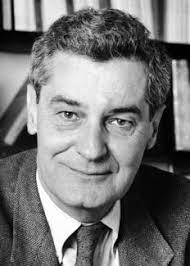
\includegraphics[width=0.24\textwidth]{./figures/aula11_fig1.jpeg}} \quad
        \subfloat[Thomas Sargent (1943 - )\label{fig1b}]{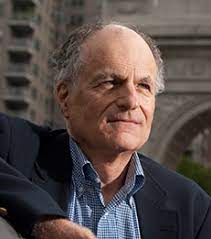
\includegraphics[width=0.3\textwidth]{./figures/aula11_fig2.jpeg}} \quad 
        \subfloat[Robert Barro (1944 - )\label{fig1c}]{
\includegraphics[width=0.25\textwidth]{./figures/aula11_fig3.jpeg}}
        \caption{Economistas novo-clássicos.}
        \label{fig1p1}
    \end{figure}
\end{frame}

\begin{frame}{Introdução}
    \begin{figure}
        \centering
        \subfloat[Edward Prescott (1940 - 2022)\label{fig2a}]{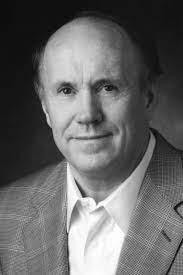
\includegraphics[width=0.2\textwidth]{./figures/aula11_fig4.jpeg}} \quad
        \subfloat[Neil Wallace (1939 - )\label{fig2b}]{
\includegraphics[width=0.3\textwidth]{./figures/aula11_fig5.jpeg}}
        \caption{Economistas novo-clássicos.}
        \label{fig1p2}
    \end{figure}
\end{frame}

\begin{frame}{Introdução}
    \begin{itemize}
        \item Objetivos deste bloco:
        \bigskip
        \begin{enumerate}
            \item Discutir as proposições teóricas centrais subjacentes aos modelos novo-clássicos
            \bigskip
            \item Considerar a teoria novo-clássica de ciclos de negócios
            \bigskip
            \item Discutir as principais implicações de política econômica que derivam da abordagem novo-clássica
            \bigskip
            \item Analisar o impacto da escola novo-clássica no desenvolvimento da macroeconomia
        \end{enumerate}
    \end{itemize}
\end{frame}

\section{Estrutura dos modelos novo-clássicos}
\subsection{Estrutura dos modelos: Introdução}
\begin{frame}{Introdução}
    \begin{itemize}
        \item Principais características:
        \bigskip
        \begin{enumerate}
            \item Sustentação da teoria macro com microfundamentações na abordagem de teoria da escolha neoclássica em um sistema de equilíbrio geral Walrasiano - \textcolor{purple}{microfundamentação da macroeconomia}
            \bigskip
            \item Hipótese neoclássica de que \textcolor{purple}{agentes são racionais} - i.e., são otimizadores contínuos sujeitos às restrições que se deparam
            \bigskip
            \item Agentes não sofrem de ilusão monetária e, portanto, \textcolor{purple}{apenas magnitudes reais (preços relativos) importam para decisões otimizadoras}
            \bigskip
            \item Flexibilidade completa e contínua de preços e salários assegura que mercados continuamente se equilibram à medida que os agentes exaurem todos os ganhos mútuos derivados do comércio - nenhuma oportunidade rentável é inexplorada
        \end{enumerate}
    \end{itemize}
\end{frame}

\begin{frame}{Introdução}
    \begin{itemize}
        \item Hipóteses $\Rightarrow$ variações na quantidade de moeda deveriam ser neutras e magnitudes reais independentes das variáveis nominais
        \bigskip
        \item Evidência empírica mostra que existem correlações positivas (ao menos no curto prazo) entre:
        \bigskip
        \begin{enumerate}
            \item PIB real e nível de preços - OA positivamente inclinada
            \bigskip
            \item Variações na oferta nominal de moeda e PIB real
            \bigskip
            \item Correlações negativas entre inflação e desemprego - curva de Phillips
        \end{enumerate}
        \bigskip
        \item \hlight{Empiricamente a moeda não parece ser neutra no curto prazo}
    \end{itemize}
\end{frame}

\begin{frame}{Introdução}
    \begin{itemize}
        \item \textcolor{purple}{Problema de Lucas:} neutralidade da moeda prevista pela teoria clássica/neoclássica $\times$ evidência empírica de não-neutralidades da moeda
        \bigskip
        \item \hlight{\emph{Expectations and the neutrality of money} (Lucas, 1972)}: substitui hipótese clássica de que agentes possuem informação perfeita pela hipótese de \textcolor{purple}{informação imperfeita}
        \bigskip
        \item Abordagem novo-clássica - aceitação conjunta de três sub-hipóteses:
        \bigskip
        \begin{enumerate}
            \item \textcolor{blue}{Hipótese de expectativas racionais}
            \bigskip
            \item \textcolor{blue}{Hipótese de equilíbrio de mercado contínuo}
            \bigskip
            \item \textcolor{blue}{Hipótese de oferta agregada de Lucas}
        \end{enumerate}        
    \end{itemize}
\end{frame}

\begin{frame}{Introdução}
    \begin{figure}
        \centering
        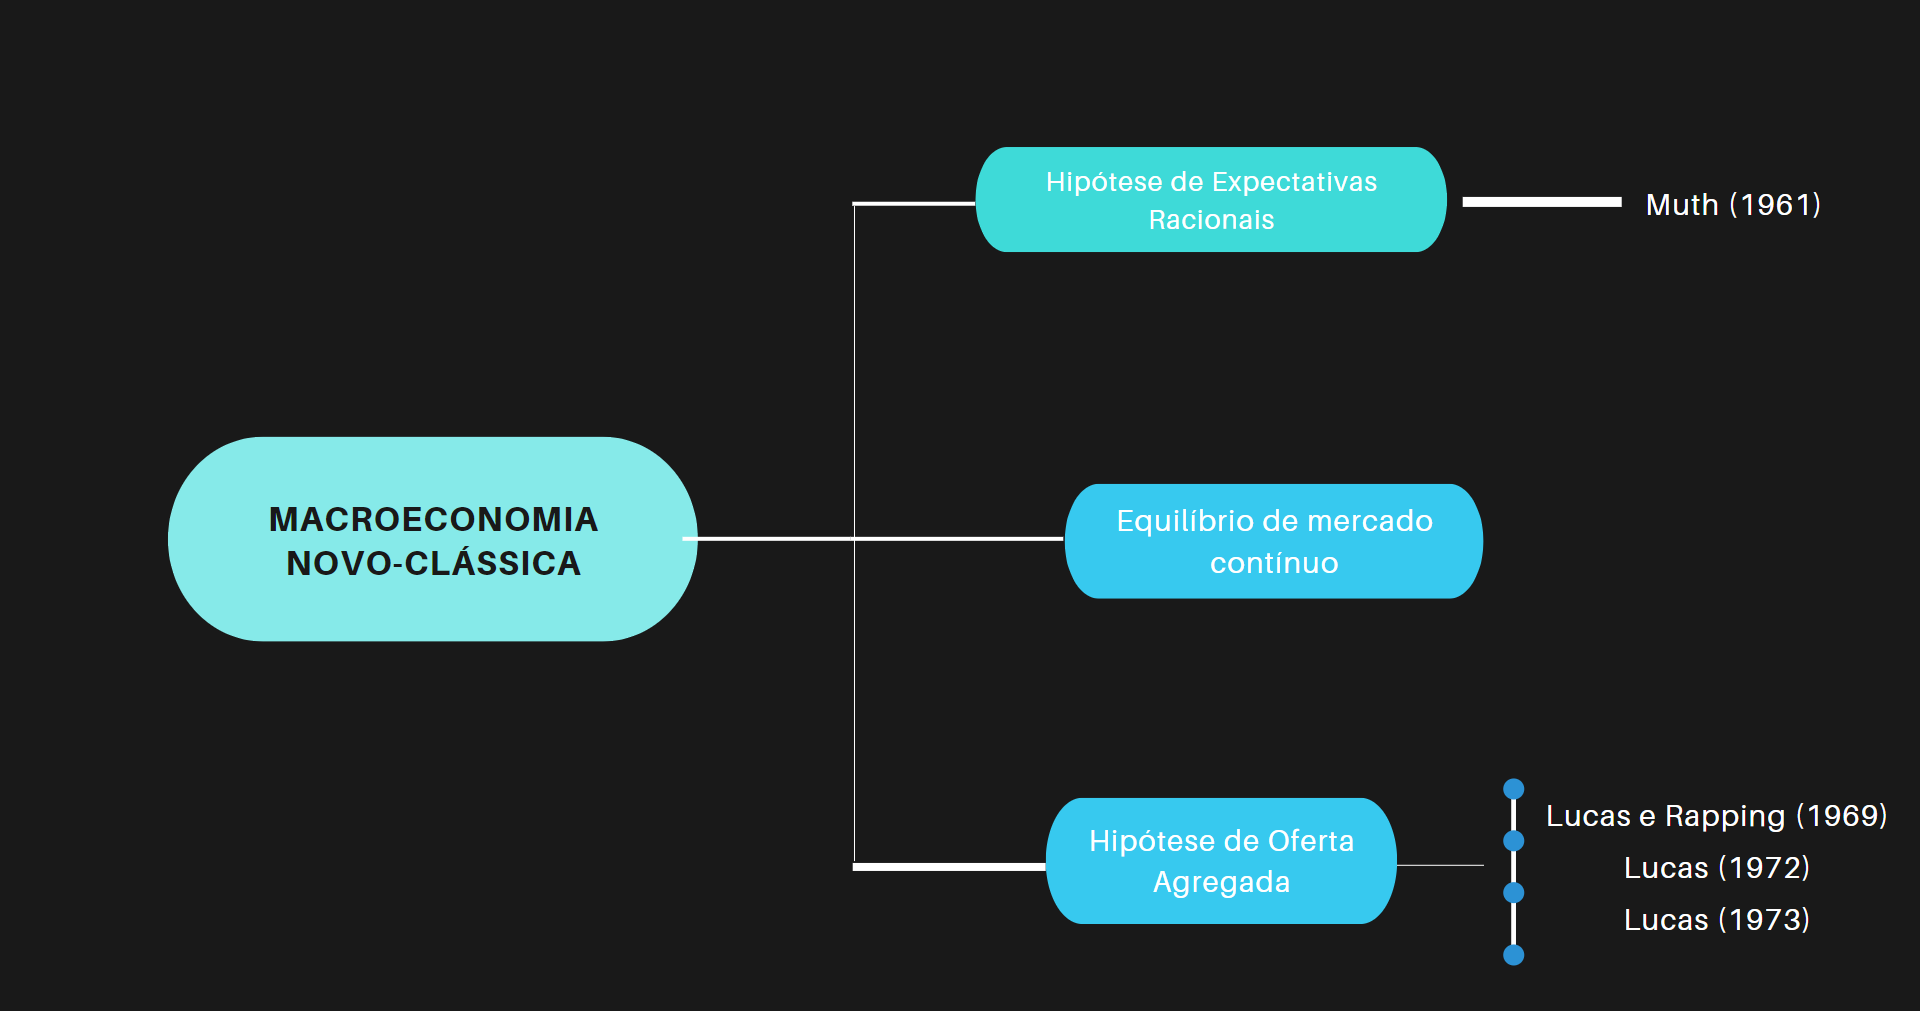
\includegraphics[width=0.85\textwidth]{./figures/aula11_fig6.PNG}
        \caption{Estrutura dos modelos novos-clássicos. Fonte: Snowdon e Vane (2005).}
        \label{fig3}
    \end{figure}
\end{frame}

\subsection{Hipótese das expectativas racionais}
\begin{frame}{Expectativas racionais}
    \begin{itemize}
        \item Em um contexto de teoria micro:
        
        \NB{
            Expectativas, dado que s\~{a}o predi\c{c}\~{o}es a partir de informa\c{c}\~{o}es de eventos futuros, s\~{a}o essencialmente as mesmas que as predi\c{c}\~{o}es da teoria econ\^{o}mica relevante
            \begin{flushright}
                (John Muth, 1961).
            \end{flushright}
        }
        \bigskip
        \item As expectativas, que são subjetivas, são fundamentais ao comportamento dos agentes, e todas as atividades econômicas possuem uma dimensão expectacional/informacional
        \bigskip
        \item Por exemplo, expectativas acerca dos valores futuros de variáveis econômicas irão, claramente, influenciar as decisões de oferta e demanda
    \end{itemize}
\end{frame}

\begin{frame}{Expectativas racionais}
    \NB{
        Dado que praticamente todas as decis\~{o}es econ\^{o}micas envolvem tomar a\c{c}\~{o}es hoje para recompensas incertas no futuro, as expectativas com rela\c{c}\~{a}o ao futuro s\~{a}o cruciais para o processo decis\'{o}rio
        \begin{flushright}
            (Carter e Maddock, 1984).
        \end{flushright}            
    }
    \begin{itemize}
        \item Exemplo: expectativas de inflação influenciam o comportamento dos agentes nos processos de barganhas salariais entre sindicatos e empregadores
        \bigskip
        \item Se o negociador por parte dos sindicatos subestimar a taxa de inflação prevalente ao longo do período negociado para o contrato salarial, então, os trabalhadores irão sofrer um aumento salarial nominal, mas um corte de salários reais
    \end{itemize}
\end{frame}

\begin{frame}{Expectativas racionais}
    \begin{itemize}
        \item Expectativa de alguma variável econômica relevante não precisa estar restrita a um único valor previsto, pode \hlight{envolver uma distribuição de probabilidades dos resultados possíveis}
        \bigskip
        \item Duas questões fundamentais para incorporação de expectativas aos modelos econômicos:
        \bigskip
        \begin{enumerate}
            \item Como indivíduos adquirem, processam e utilizam as informações para formar suas expectativas a respeito das variáveis relevantes?
            \bigskip
            \item Qual hipótese expectacional devemos usar nos modelos macroeconômicos?
        \end{enumerate}
    \end{itemize}
\end{frame}

\begin{frame}{Expectativas racionais}
    \begin{itemize}
        \item 1970s: hipótese de expectativas racionais (HER) substituiu a hipótese de expectativas adaptativas como forma dominante de modelar \hlight{expectativas endógenas}
        \bigskip
        \item Teoria Geral: destaca a importância das expectativas para a compreensão de instabilidades macroeconômicas. No entanto, expectativas são \textcolor{red}{exógenas}, determinadas por \emph{animal spirits}
        \bigskip
        \item Vantagem da HER sobre hipóteses alternativas (não-racionais): estas últimas envolvem erros sistemáticos, uma situação que não condiz com os cálculos racionais dos agentes econômicos previstas pelos modelos neoclássicos ortodoxos
    \end{itemize}
\end{frame}

\begin{frame}{Expectativas racionais}
    \begin{itemize}
        \item HER apresentada de diversas formas ao longo do tempo. Destacaremos a distinção entre \textcolor{purple}{versão fraca} e \textcolor{blue}{versão forte}
        \bigskip        
        \item \textcolor{purple}{Versão fraca:} ao formar previsões ou expectativas acerca do valor futuro de uma variável, agentes racionais utilizarão da melhor forma possível (mais eficiente) todas as informações disponíveis publicamente acerca dos fatores que acreditam determinar esta variável
        \bigskip
        \item I.e., assume-se que as expectativas são formadas `racionalmente' em linha com o comportamento de maximização de utilidade por parte dos agentes econômicos individuais
        \bigskip
        \item E.g., se agentes acreditam que a taxa de inflação é determinada pela taxa de expansão monetária, utilizarão da maneira mais eficiente possível as informações publicamente disponíveis a respeito das taxas de expansão monetária quando forem formar suas expectativas de taxas de inflação futuras
    \end{itemize}
\end{frame}

\begin{frame}{Expectativas racionais}
    \begin{itemize}
        \item \textcolor{blue}{Versão forte:} expectativas subjetivas dos agentes acerca das variáveis irão coincidir com a esperança matemática condicional verdadeira ou objetiva destas variáveis
        \bigskip
        \item Para o exemplo de formação de expectativas a respeito das taxas de inflação futuras ($\dot{P}_t^e$), formalmente:
        \begin{equation}
            \dot{P}_t^e = \mathbb{E}(\dot{P}_t|\Omega_{t-1}).
            \label{eq1}
        \end{equation}
        \bigskip
        \item $\dot{P}_t$ é a taxa de inflação observada, $\mathbb{E}(\dot{P}_t|\Omega_{t-1})$ é a expectativa racional da taxa de inflação sujeita à informação disponível até o período anterior ($\Omega_{t-1}$) - conjunto de informação
        \bigskip
        \item \hlight{expectativas racionais não significam que agentes podem prever o futuro de maneira exata}
        \bigskip
        \item \hlight{Expectativas racionais não é o mesmo que previsão perfeita}
    \end{itemize}
\end{frame}

\begin{frame}{Expectativas racionais}
    \begin{itemize}
        \item \hlight{Expectativas dos agentes com respeito a uma dada variável devem ser consistentes com as predições do modelo teórico}:
        
        \NB{
            As previs\~{o}es feitas pelo agente dentro do modelo n\~{a}o podem ser piores que as previs\~{o}es feitas pelo economista que possui o modelo
        
        \begin{flushright}
            (Sargent, 1987).
        \end{flushright}
        }
        \bigskip
        \item Portanto, ao formar suas expectativas racionais a respeito da taxa de inflação futura, os agentes deverão levar em consideração o que eles acreditam ser o modelo macroeconômico `correto' da economia
    \end{itemize}
\end{frame}

\begin{frame}{Expectativas racionais}
    \begin{itemize}
        \item Agentes cometerão erros em suas previsões, dado que a informação disponível será incompleta - elemento essencial do modelo de surpresas monetárias de Lucas
        \bigskip
        \item No entanto, estes erros de previsão serão não relacionados ao conjunto de informação no período em que a expectativa foi formada
        \bigskip
        \item Com expectativas racionais, as expectativas dos agentes a respeito de variáveis econômicas serão corretas na média, i.e., serão iguais aos valores verdadeiros
    \end{itemize}
\end{frame}

\begin{frame}{Expectativas racionais}
    \begin{itemize}
        \item \hlight{Agentes não formarão expectativas que são sistematicamente incorretas (viesadas) ao longo do tempo}
        \bigskip
        \item Se expectativas fossem sistematicamente viesadas, agentes iriam aprender com erros de previsão e mudar a forma com que formam expectativas, eliminando estes erros sistemáticos
        \bigskip
        \item De maneira mais formal, HER implica que:
        \begin{equation}
            \dot{P}_t^e = \dot{P}_t + \varepsilon_t,
            \label{eq2}
        \end{equation}
        onde $\dot{P}_t^e$ é a taxa de inflação esperada entre $t$ e $t+1$, $\dot{P}_t$ é a taxa de inflação observada entre $t$ e $t+1$, e $\varepsilon_t$ é um termo de erro aleatório
    \end{itemize}
\end{frame}

\begin{frame}{Expectativas racionais}
    \begin{itemize}
        \item Hipóteses com relação ao termo de erro:
        \bigskip
        \begin{enumerate}
            \item Possui média zero
            \medskip
            \item Não-correlacionado com o conjunto de informação disponível no período em que as expectativas são formadas. Não fosse este o caso, os agentes econômicos não estariam explorando completamente as informações disponíveis
        \end{enumerate}
        \bigskip
        \item Em resumo, os erros de previsão de expectativas formadas racionalmente serão:
        \bigskip
        \begin{enumerate}
            \item Aleatórios com média zero
            \medskip
            \item Não correlacionados com os erros feitos nos períodos anteriores, revelando nenhum padrão discernível: i.e., serão serialmente não-correlacionados ao longo do tempo
            \medskip
            \item Possuirão a menor variância quando comparados com qualquer outro método de previsão
        \end{enumerate}
        \bigskip
        \item \hlight{Expectativas racionais são a forma mais precisa e eficiente de formação de expectativas}
    \end{itemize}
\end{frame}

\begin{frame}{Expectativas racionais}
    \begin{itemize}
        \item \textcolor{blue}{Expectativas racionais} $\times$ \textcolor{purple}{expectativas adaptativas}.
        \bigskip
        \item Curva de Phillips aumentada por expectativas (monetarista): agentes baseiam suas expectativas a respeito dos valores futuros das variáveis apenas em seus valores passados
        \bigskip
        \item Um dos principais problemas com essa abordagem `backward-looking' de formação de expectativas é que, até que a variável prevista seja estável por um período de tempo considerável, as expectativas formadas serão repetidamente erradas
    \end{itemize}
\end{frame}

\begin{frame}{Expectativas racionais}
    \begin{itemize}
        \item E.g., na hipótese aceleracionista, se o desemprego é mantido abaixo da taxa natural, a inflação irá acelerar e as expectativas inflacionárias serão viesadas em uma direção descendente
        \bigskip
        \item Este problema resulta de:
        \bigskip
        \begin{enumerate}
            \item Hipótese de que agentes ajustam apenas parcialmente suas expectativas por uma fração do último erro cometido
            \medskip
            \item A incapacidade dos agentes em levar em consideração as informações adicionais disponíveis que não sejam os valores passados da variável considerada, apesar de fazerem erros repetidos            
        \end{enumerate}
        \bigskip
        \item \textcolor{blue}{Abordagem `forward-looking'}: expectativas racionais são baseadas no uso de toda informação pública disponível, com a implicação crucial da versão forte sendo que os agentes econômicos não irão formar suas expectativas de maneira sistematicamente errada ao longo do tempo - \hlight{expectativas serão não-viesadas}        
    \end{itemize}
\end{frame}

\begin{frame}{Expectativas racionais: principais críticas}
    \begin{itemize}
        \item[(1)] Custos (em termos de tempo, esforço e monetários) de aquisição e processamento de todas as informações publicamente disponíveis para prever os valores futuros de uma variável econômica.
        \bigskip
        \item Importante notar que a versão fraca da HER não requer que os agentes econômicos usem \textcolor{purple}{todas} as informações publicamente disponíveis.
        \bigskip
        \item Dados os custos envolvidos em adquirir e processar informação, é improvável que os agentes utilizarão toda a informação disponível publicamente.
        \bigskip
        \item Proponentes da versão fraca argumentam que agentes econômicos racionais tem um incentivo a fazer o `melhor' uso de toda a informação publicamente disponível ao formar suas expectativas.
    \end{itemize}
\end{frame}

\begin{frame}{Expectativas racionais: principais críticas}
    \begin{itemize}
        \item Dito de outra forma, \textcolor{purple}{sob a versão fraca da HER, os agentes têm um incentivo a usar o conjunto de informação disponível até o ponto em que o benefício marginal (em termos de melhoras de precisão na previsão da variável relevante) seja igual ao custo marginal (em termos de aquisição e processamento de toda a informação pública disponível)}.
        \bigskip
        \item Neste caso, as expectativas seriam menos eficientes do que seriam se toda a informação disponível fosse utilizada.
        \bigskip
        \item Além disso, a versão fraca não requer que todos os agentes individuais diretamente adquiram e processem as informações disponíveis eles mesmos.
        \bigskip
        \item Eles podem `consumir' informação de forma indireta, e.g., via previsões publicadas e comentários nas mídias.
        \bigskip
        \item Dado que as previsões frequentemente diferem, o problema neste caso seria discernir qual é a visão `correta'.
    \end{itemize}
\end{frame}

\begin{frame}{Expectativas racionais: principais críticas}
    \begin{itemize}
        \item[(2)] Como os agentes podem, de fato, obter conhecimento a respeito do modelo `correto' da economia, dado que até economistas apresentam divergências consideráveis a esse respeito?
        \bigskip
        \item Essa é uma objeção bem mais grave com relação à HER.
        \bigskip
        \item No entanto, é importante notar que a \textcolor{blue}{versão forte da HER} não requer que os agentes econômicos conheçam, de fato, o modelo correto do sistema econômico.
        \bigskip
        \item O que a hipótese implica é, simplesmente, que os agentes não irão formar expectativas que sejam sistematicamente erradas ao longo do tempo.
        \bigskip
        \item Dito de outra forma, as expectativas serão similares àquelas formadas ``como se'' os agentes conhecessem o modelo correto no sentido em que serão não-viesadas e distribuídas aleatoriamente ao longo do tempo.
    \end{itemize}
\end{frame}

\begin{frame}{Expectativas racionais: principais críticas}
    \begin{itemize}
        \item Para alguns economistas, estes argumentos não são convincentes. Dados os problemas relacionados aos custos de aquisição e processamento de todas as informações disponíveis, é possível que agentes formem expectativas que sejam sistematicamente incorretas.
        \bigskip
        \item Existem algumas evidências que sugerem que agentes, de fato, cometem erros sistemáticos em suas expectativas - Lovell, 1986.
        \bigskip
        \item[(3)] A terceira crítica, muito associada à escola pós-Keynesiana, é relacionada aos problemas de formação de expectativas em um mundo inerentemente incerto.
        \bigskip
        \item Para fundamentalistas Keynesianos, a principal contribuição de Keynes é colocar o problema relacionado à \textcolor{purple}{incerteza} no centro da discussão macroeconômica.
    \end{itemize}
\end{frame}

\begin{frame}{Expectativas racionais: principais críticas}
    \begin{itemize}
        \item Na visão pós-Keynesiana, o mundo é \textcolor{purple}{não-ergódico}. Isto é, cada evento histórico é único e não-repetitivo.
        \bigskip
        \item Em tais situações, as regras de probabilidade não são aplicáveis.
        \bigskip
        \item Pós-Keynesianos, portanto, argumentam que é importante seguirmos Keynes (1921) e Knight (1933) e distinguir entre situações envolvendo \textcolor{blue}{risco} de situações envolvendo \textcolor{purple}{incerteza}.
        \bigskip
        \item Diz-se que uma situação envolve \textcolor{blue}{risco} se a aleatoriedade com a qual um agente econômico se depara se apresenta sob a forma de \emph{probabilidades objetivas} exogenamente especificadas ou cientificamente calculáveis. Ou seja, a distribuição de probabilidades é conhecida - e.g., apostas baseadas em roletas ou um par de dados.
        \bigskip
        \item Por outro lado, diz-se que uma situação envolve \textcolor{purple}{incerteza} se a aleatoriedade se apresenta sob a forma de eventos possíveis alternativos. Neste caso, não há possibilidades de formular qualquer distribuição de probabilidades significativa - e.g., apostas em uma corrida de cavalos, ou comprar ou não seguros contra terremotos.
    \end{itemize}
\end{frame}

\begin{frame}{Expectativas racionais: principais críticas}
    \begin{itemize}
        \item Como a HER assume que os agentes econômicos podem formular distribuições de probabilidades dos resultados de várias mudanças e situações econômicas, configura-se um ambiente de risco.
        \bigskip
        \item Nos modelos novo-clássicos, o problema de incerteza fundamental é ignorado, dado que Lucas (1977) interpreta os ciclos de negócios como instâncias repetidas de eventos essencialmente similares.
        \bigskip
        \item Portanto, no mundo ergódico de Lucas, distribuições de probabilidade significativas podem ser medidas por agentes econômicos racionais.
        \bigskip
        \item No entanto, para os pós-Keynesianos, o mundo `real' é caracterizado por uma incerteza fundamental e, então, conclusões obtidas em modelos usando as HER são `inúteis'.
    \end{itemize}
\end{frame}

\begin{frame}{Expectativas racionais}
    \begin{itemize}
        \item Em 2003, o Bank of England analisou os vários fatores que influenciam expectativas em um survey sobre inflação. Sumário dos resultados:
        \begin{enumerate}
            \item Desagregação dos dados revelam que pessoas e grupos diferentes possuem diferentes atitudes com relação à inflação.
            \bigskip
            \item As expectativas de grupos `profissionais' estão clusterizadas ao redor da expectativa média.
            \bigskip
            \item Pessoas mais novas possuem uma expectativa de inflação mais baixa que pessoas mais velhas.
            \bigskip
            \item Detentores de hipotecas possuem expectativas inflacionárias mais baixas que entrevistados que alugam acomodações.
            \bigskip
            \item Pessoas no sul da Grã-Bretanha possuem expectativas inflacionárias mais elevadas que entrevistados que vivem no norte.
            \bigskip
            \item A experiência inflacionária ao longo da vida dos entrevistados influencia as expectativas de inflação.
        \end{enumerate}
    \end{itemize}
\end{frame}

\begin{frame}{Expectativas racionais}
    \begin{itemize}
        \item Portanto, expectativas inflacionárias são influenciadas por idade, localização geográfica, educação e ocupação, e status de habitação.
        \bigskip
        \item E.g., indivíduos que viveram ao longo do período da `Grande Inflação' dos anos 1970 ainda não removeram completamente este passado inflacionário.
    \end{itemize}
\end{frame}

\subsection{Equilíbrio contínuo de mercado}

\begin{frame}{Equilíbrio contínuo de mercado}
    \begin{itemize}
        \item Seguindo a tradição Walrasiana, um segundo elemento crucial aos modelos novo-clássicos é que todos os mercados do sistema econômico continuamente se equilibram.
        \bigskip
        \item Em cada ponto do tempo, todos os resultados observados são vistos como `equilíbrios de mercado', e são o resultado das respostas ótimas de oferta e demanda dos agentes econômicos às suas percepções de preços.
        \bigskip
        \item Portanto, a economia é vista como \textcolor{purple}{em estado de contínuo equilíbrio (de curto e longo prazo)}.
        \bigskip
        \item Modelos novo-clássicos são, consequentemente, referidos como modelos de `equilíbrio'.
        \bigskip
        \item Equilíbrio no sentido em que todos os agentes em uma economia de mercado fizeram escolhas que otimizam seus objetivos sujeitos às restrições que lhes são impostas.
    \end{itemize}
\end{frame}

\begin{frame}{Equilíbrio contínuo de mercado}
    \begin{itemize}
        \item Em modelos de equilíbrio de mercado, os agentes econômicos (trabalhadores, consumidores e firmas) são tomadores de preços.
        \bigskip
        \item Nesta estrutura de mercado, as firmas podem decidir apenas a quantidade ótima (maximizadora de lucro) produzida dados os preços determinados pelo mercado (RMg = CMg).
        \bigskip
        \item Na ausência de externalidades, o equilíbrio de mercado com preços de mercado determinados pelas forças de oferta e demanda, é um ótimo de Pareto e maximiza o excedente total (excedente do consumidor + excedente do produtor).
    \end{itemize}
\end{frame}

\begin{frame}{Equilíbrio contínuo de mercado}
    \begin{figure}
        \centering
        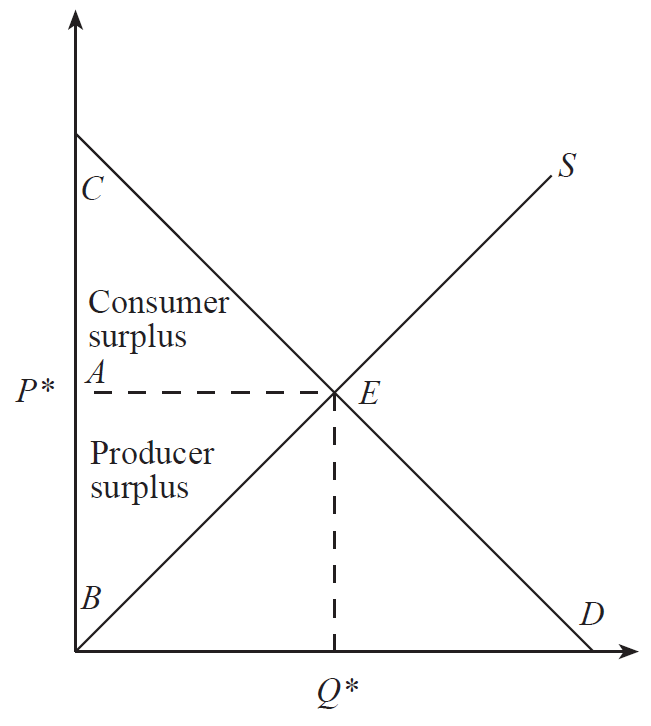
\includegraphics[width=0.5\textwidth]{./figures/aula11_fig7.PNG}
        \caption{Equilíbrio de mercado competitivo e bem-estar. Fonte: Snowdon e Vane (2005).}
        \label{fig4}
    \end{figure}
\end{frame}

\begin{frame}{Equilíbrio contínuo de mercado}
    \begin{itemize}
        \item Na Figura \ref{fig4} podemos ver que um equilíbrio de mercado ($P^*,Q^*)$ maximiza o excedente total do consumidor e produtor (área BCE).
        \bigskip
        \item Neste caso, todos os ganhos mútuos do comércio foram exauridos pelos agentes econômicos utilizando todos seus recursos.
        \bigskip
        \item No caso em que os preços (quantidades) são diferentes dos valores de equilíbrio de mercado, teremos uma perda de bem estar.
        \bigskip
        \item Na Figura \ref{fig5}, $P_1(Q_1)$ resulta em uma perda de bem estar dada pela área FEI e $P_2(Q_2)$ por GEH.
    \end{itemize}
\end{frame}

\begin{frame}{Equilíbrio contínuo de mercado}
    \begin{figure}
        \centering
        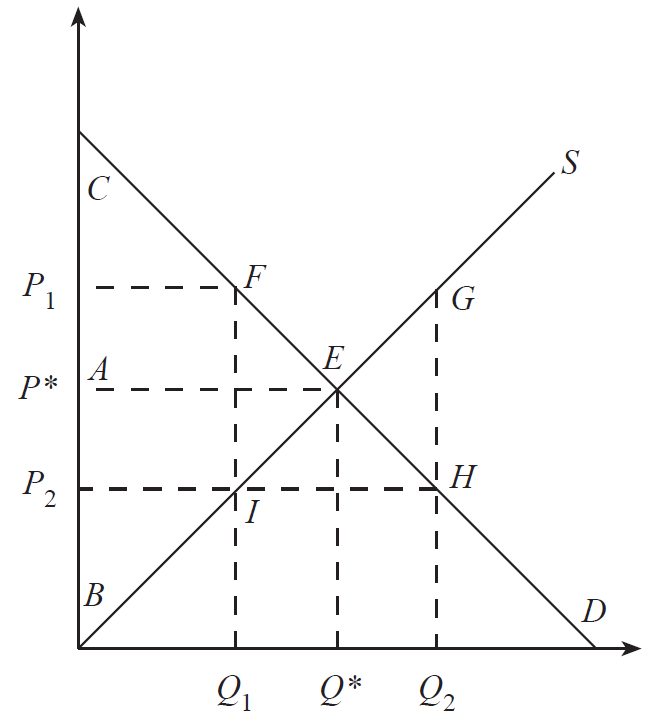
\includegraphics[width=0.5\textwidth]{./figures/aula11_fig8.PNG}
        \caption{Perda de bem-estar se o preço estiver acima ou abaixo do nível competitivo. Fonte: Snowdon e Vane (2005).}
        \label{fig5}
    \end{figure}
\end{frame}

\begin{frame}{Equilíbrio contínuo de mercado}
    \begin{itemize}
        \item É importante ressaltar que \textcolor{purple}{as posições das curvas de oferta e demanda e, portanto, os preços e quantidades de equilíbrio de mercado, são influenciadas pelas expectativas dos agentes}.
        \bigskip
        \item Dado que até expectativas formadas racionalmente podem estar erradas devido a informação incompleta, isso significa que, até que os agentes obtenham informações mais precisas, um equilíbrio observável de mercado irá diferir de um equilíbrio de informação completa.
        \bigskip
        \item No entanto, como os agentes estão fazendo o melhor possível com as informações adquiridas, temos um estado de equilíbrio em todos os períodos:
        \[
        \text{RACIONALIDADE} \implies \text{OTIMIZAÇÃO} \implies \text{EQUILÍBRIO}.
        \]
    \end{itemize}
\end{frame}

\begin{frame}{Equilíbrio contínuo de mercado}
    \begin{itemize}
        \item A hipótese de equilíbrio contínuo de mercado é a mais central e controversa subjacente aos modelos novo-clássicos - implica que os preços são flexíveis para se ajustarem de forma instantânea de maneira a assegurar o equilíbrio nos mercados.
        \bigskip
        \item Este pressuposto contrasta tanto com a abordagem Keynesiana quanto monetarista.
        \bigskip
        \item Vimos que há uma divergência entre Keynesianos e monetaristas acerca do tempo necessário para a economia atingir o equilíbrio nos mercados.
    \end{itemize}
\end{frame}

\begin{frame}{Equilíbrio contínuo de mercado}
    \begin{itemize}
        \item \textcolor{red}{Modelos Keynesianos incorporam o pressuposto de que os mercados podem não se equilibrar dado o lento ajuste dos preços, de forma que a economia é vista como um possível estado de contínuo desequilíbrio}.
        \bigskip
        \item \textcolor{purple}{Modelos monetaristas assumem que os preços se ajustam relativamente rápido para equilibrar os mercados, ao mesmo tempo que admitem que a economia pode estar em desequilíbrio no curto prazo. No longo prazo, a economia automaticamente retorna a um estado de equilíbrio macroeconômico ao nível natural de emprego e produto}.
    \end{itemize}
\end{frame}

\begin{frame}{Equilíbrio contínuo de mercado}
    \begin{itemize}
        \item O pressuposto de equilíbrio contínuo de mercado é bem mais controverso que HER.
        \bigskip
        \item Como veremos mais adiante, \textcolor{purple}{novos-Keynesianos} fornecem vários argumentos para explicar porque tanto preços quanto salários se ajustam lentamente para equilibrar os mercados após o sistema ser perturbado por algum choque.
        \bigskip
        \item Sérias objeções podem ser levantadas a respeito do realismo deste pressuposto novo-clássico, principalmente quando tratamos mercado de trabalho.
        \bigskip
        \item Para \textcolor{blue}{novos-clássicos}, qualquer pessoa disposta a trabalhar consegue encontrar emprego ao nível de salário de equilíbrio de mercados.
        \bigskip
        \item Portanto, o desemprego é um fenômeno inteiramente voluntário.
    \end{itemize}
\end{frame}

\begin{frame}{Equilíbrio contínuo de mercado}
    \begin{itemize}
        \item No entanto, dadas considerações de salário-eficiência (que veremos mais adiante) pode-se argumentar que é tanto lucrativo quanto racional para um firma pagar um salário-eficiência acima do nível de equilíbrio competitivo.
        \bigskip
        \item Em uma situação como essa, o equilíbrio no mercado de trabalho pode ocorrer onde a oferta excede a demanda, com a existência de desemprego involuntário como um fenômeno de equilíbrio.
    \end{itemize}
\end{frame}

\subsection{A hipótese de oferta agregada}
\begin{frame}{Hipótese de oferta agregada}
    \begin{itemize}
        \item Com relação à hipótese de oferta agregada, duas abordagens principais podem ser identificadas.
        \bigskip
        \item Subjacentes a estas abordagens estão duas hipóteses microeconômicas tradicionais:
        \bigskip
        \begin{enumerate}
            \item Escolhas racionais tomadas por firmas e trabalhadores refletem comportamentos otimizadores.
            \bigskip
            \item A oferta de trabalho/produto por parte dos trabalhadores/firmas depende de preços relativos.
        \end{enumerate}
    \end{itemize}
\end{frame}

\begin{frame}{Hipótese de oferta agregada}
    \begin{enumerate}
        \item A primeira abordagem novo-clássica de oferta agregada foca na oferta de trabalho - Lucas e Rapping (1969).
        \bigskip
        \begin{itemize}
            \item Esta abordagem envolve a noção de \textcolor{purple}{elasticidade intertemporal de substituição} do lazer - um dos pilares da macroeconomia DSGE.
            \bigskip
            \item Essência: durante qualquer período, trabalhadores precisam decidir quanto tempo alocar entre trabalho e lazer.
            \bigskip
            \item Assume-se que trabalhadores tem uma noção de qual o salário real médio esperado.
            \bigskip
            \item Se salário real corrente está acima do nível médio esperado, têm um incentivo para trabalhar mais (menos tempo de lazer) no período corrente antecipando um maior tempo de lazer (trabalhar menos) no futuro, quando espera-se um salário real menor.
            \bigskip
            \item A oferta de trabalho é postulada, portanto, para responder a variações temporárias percebidas no salário real.
        \end{itemize}
    \end{enumerate}
\end{frame}

\begin{frame}{Hipótese de oferta agregada}
    \begin{itemize}
        \item No modelo de elasticidade intertemporal de substituição do lazer (substituição de lazer corrente por lazer futuro, vice-versa), variações no nível de emprego são explicados em termos de escolhas `voluntárias' dos trabalhadores que alteram sua oferta de trabalho em resposta a variações temporárias percebidas no nível de salário real.
    \end{itemize}
\end{frame}

\begin{frame}{Hipótese de oferta agregada}
    \begin{enumerate}
        \setcounter{enumi}{1}
        \item Segunda abordagem novo-clássica de oferta agregada - Lucas (1972, 1973).
        \bigskip
        \begin{itemize}
            \item Explicaremos esta abordagem focando no mercado de bens e nas decisões de oferta por parte das firmas.
            \bigskip
            \item Um elemento importante está relacionado à estrutura do conjunto de informação disponível aos produtores.
            \bigskip
            \item Assume-se que, enquanto a firma conhece o preço corrente de mercado do bem que ela produz, o nível de preços geral para outros mercados só se torna conhecido com um hiato temporal.
            \bigskip
            \item \textcolor{purple}{Modelo de surpresas inflacionárias de Lucas}.
        \end{itemize}
    \end{enumerate}
\end{frame}

\begin{frame}{Hipótese de oferta agregada}
    \begin{itemize}
        \item Quando uma firma percebe um aumento no preço corrente de mercado do bem que ela produz, ela precisa decidir se este aumento de preço reflete:
        \bigskip
        \begin{enumerate}
            \item Um deslocamento real de demanda em direção ao seu produto - neste caso a firma deve responder (racionalmente) a esse aumento de preço relativo aumentando sua produção.
            \bigskip
            \item Um aumento nominal de demanda em todos os mercados - um aumento generalizado do nível de preços não deveria requerer uma resposta de oferta.
        \end{enumerate}
        \bigskip
        \item Firmas se deparam com o que conhecemos por um \textcolor{blue}{problema de extração de sinal}: deve distinguir entre uma variação de preços absolutos ou relativos.
        \bigskip
        \item \textcolor{purple}{Quanto maior a volatilidade do nível geral de preços, mais difícil será para produtores extrair o sinal correto e menos espera-se ajustes de oferta para qualquer variação de preços}.
    \end{itemize}
\end{frame}

\begin{frame}{Hipótese de oferta agregada}
    \begin{itemize}
        \item A análise do comportamento de agentes individuais em termos de oferta de trabalho e bens levou à \textcolor{purple}{função de oferta de Lucas}:
        \begin{equation}
            Y_t = Y_t^n + \alpha(P_t - P_t^e), \qquad \alpha > 0.
            \label{eq3}
        \end{equation}
        \bigskip
        \item Em modelos novo-clássicos - HER, portanto:
        \begin{equation}
            Y_t = Y_t^n + \alpha\left(P_t - \mathbb{E}[P_t|\Omega_{t-1}]\right).
            \label{eq4}
        \end{equation}
        \bigskip
        \item A equação (\ref{eq4}) nos diz que o produto agregado desviará do seu nível natural apenas em resposta a desvios do nível de preços corrente com relação ao seu valor esperado de ER.
    \end{itemize}
\end{frame}

\begin{frame}{Hipótese de oferta agregada}
    \begin{itemize}
        \item E.g., quando o nível de preços corrente é maior que o esperado, os agentes individuais são `surpreendidos' e interpretam, de forma errônea, este aumento generalizado de preços como um aumento de preço relativo do bem que produzem - aumenta a oferta de bens e de trabalho na economia.
        \bigskip
        \item Na ausência de surpresas de preços, o produto está em seu nível natural.
        \bigskip
        \item Para qualquer nível de preços esperado, a \textcolor{purple}{curva de oferta agregada} será positivamente inclinada no plano P-Y.
        \bigskip
        \item Quanto maior o valor de $\alpha$, mais elástica será a curva de oferta agregada de Lucas e maior será o impacto sobre variáveis reais de um aumento não-antecipado no nível geral de preços.
    \end{itemize}
\end{frame}

\begin{frame}{Hipótese de oferta agregada}
    \begin{itemize}
        \item OA de Lucas (alternativa) - hiato do produto responde a desvios da inflação esperada com relação à inflação observada (i.e., a erros na formação de expectativas):
        \begin{equation}
            Y_t = Y_t^n + \alpha[\pi_t - \mathbb{E}(\pi_t|\Omega_{t-1})] + \varepsilon_t.
            \label{eq5}
        \end{equation}
        \bigskip
        \item Países com inflação estável  devem apresentar uma maior resposta de oferta a impulsos inflacionário, e vice-versa:
        \begin{quote}
            Em um país com preços estáveis como EUA, políticas que aumentam a renda nominal tendem a ter um efeito inicial maior sobre o produto real, conjuntamente a um efeito positivo pequeno sobre a taxa de inflação [...] Em contraste, em países com preços voláteis como a Argentina, variações de renda nominal são associadas com movimentos iguais e contemporâneos sobre os preços com nenhum efeito identificável sobre produto real.
        \end{quote}
        \begin{flushright}
            (Lucas, 1973).
        \end{flushright}
    \end{itemize}
\end{frame}

\begin{frame}{Hipótese de oferta agregada}
    \begin{itemize}
        \item Podemos reformular a equação (\ref{eq5}) para incluir um termo defasado do hiato do produto - Lucas (1973) em trabalho empírico para lidar com problema da persistência (correlação serial) nos movimentos dos agregados econômicos:
        \begin{equation}
            Y_t = Y_t^n + \alpha[P_t - \mathbb{E}(P_t|\Omega_{t-1})] + \beta(Y_{t-1}-Y_{t-1}^n) + \varepsilon_t.
            \label{eq6}
        \end{equation}
        \bigskip
        \item Pela \textcolor{purple}{lei de Okun} (relação estável negativa entre desemprego e PIB), a equação de oferta agregada de Lucas pode ser vista como uma representação alternativa da \textcolor{blue}{curva de Phillips aumentada por expectativas racionais}:
        \begin{equation}
            \pi_t = \mathbb{E}[\pi_t|\Omega_{t-1}] - \varphi(U_t - U_t^n) + \varepsilon_t, \qquad \varphi > 0.
            \label{eq7}
        \end{equation}
    \end{itemize}
\end{frame}

\begin{frame}{Hipótese de oferta agregada}
    \begin{itemize}
        \item Portanto:
        \begin{equation}
            U_t = U_t^n - \frac{1}{\varphi}(\pi_t - \mathbb{E}[\pi_t|\Omega_{t-1}]).
            \label{eq8}
        \end{equation}
        \bigskip
        \item \textcolor{purple}{Uma surpresa inflacionária leva a uma redução temporária do desemprego abaixo do seu nível natural}.
        \bigskip
        \item Nas equações anteriores, uma variável real está relacionada a uma variável nominal.
        \bigskip
        \item No entanto, \textcolor{blue}{a dicotomia clássica só não é observada quando uma variação na variável nominal for não-antecipada (`surpresa')}.
        \bigskip
        \item Essa distinção entre variações monetárias antecipadas e não-antecipadas é um elemento de todos os modelos com ER desenvolvidos durantes os anos 1970s para explicar a não-neutralidade da moeda em trade-offs de curto prazo.
    \end{itemize}
\end{frame}

\section{Bibliografia}
\begin{frame}{\emoji{books} Bibliografia}
    \begin{itemize}   
        \item ABEL, A.; BERNANKE, B.; CROUSHORE, D. Macroeconomics. 9.ed. Pearson Prentice Hall, 2017\medskip        
        \item ANDO, A.; MODIGLIANI, F. The Relative Stability of Monetary Velocity and the Investment Multiplier, American Economic Review, 1956 \medskip
        \item BLANCHARD, O. Macroeconomia. 7.ed. São Paulo: Pearson Education do Brasil, 2017\medskip                     
        \item CULBERTSON, J.M. FRIEDMAN on the Lag in Effect of Monetary Policy, Journal of Political Economy \medskip
        \item CULBERTSON, J.M. The Lag in Effect on Monetary Policy: Reply, Journal of Political Economy, 1961 \medskip
        \item DE PRANO, M.; MAYER, T. Tests of the Relative Importance of Autonomous Expenditure and Money, American Economic Review, 1965 \medskip
        \item FRIEDMAN, M. The Quantity Theory of Money, A Restatement, in M. FRIEDMAN (ed.), Studies in the Quantity Theory of Money, Chicago: University of Chicago Press, 1956 \medskip
        \item FRIEDMAN, M. The Supply of Money and Changes in Prices and Output, reprinted in The Optimum Quantity of Money and Other Essays, Chicago: Aldine, 1958 \medskip        
    \end{itemize}
\end{frame}

\begin{frame}{\emoji{books} Bibliografia}
    \begin{itemize}                        
        \item FRIEDMAN, M. The Demand for Money – Some Theoretical and Empirical Results, Journal of Political Economy, 1959 \medskip
        \item FRIEDMAN, M. The Role of Monetary Policy, American Economic Review, 1968 \medskip
        \item FRIEDMAN, M. Money: Quantity Theory, in D. Sills (ed.), The International Encyclopedia of the Social Sciences, New York: Macmillan Free Press, 1968 \medskip
        \item FRIEDMAN, M. Nobel Lecture: Inflation and Unemployment, Journal of Political Economy, 1977 \medskip
        \item FRIEDMAN, M.; MEISELMAN, D. The Relative Stability of Monetary Velocity and the Investment Multiplier in the United States, 1897–1958, in Commission on Money and Credit: Stabilization Policies, Englewood Cliffs, NJ: Prentice-Hall, 1963 \medskip
        \item FRIEDMAN, M.; SCHWARTZ, A.J. A Monetary History of the United States, 1867–1960, Princeton: Princeton University Press, 1963 \medskip
        \item KAREKEN, J.; SOLOW, R.N. Monetary Policy: Lags versus Simultaneity, in Commission on Money and Credit: Stabilization Policies, Englewood Cliffs, NJ: Prentice-Hall, 1963 \medskip        
    \end{itemize}
\end{frame}

\begin{frame}{\emoji{books} Bibliografia}
    \begin{itemize}                        
        \item MCDONALD, J.F. Rethinking Macroeconomics: a history of economic thought perspective. 2.ed. Routledge, 2022\medskip
        \item PHELPS, E.S. Phillips Curves, Expectations of Inflation and Optimal Unemployment Over Time, Economica, 1967 \medskip
        \item PHELPS, E.S. Money Wage Dynamics and Labour Market Equilibrium, Journal of Political Economy, 1968 \medskip
        \item ROGERSON, R. Theory Ahead of Language in the Economics of Unemployment, Journal of Economic Perspectives, 1997 \medskip
        \item SNOWDON, B.; VANE, H.R. \emph{Modern Macroeconomics: its Origins, Development and Current State}. Northampton, MA: Edward Elgar, 2005\medskip        
        \item STIGLITZ, J.E. Reflections on the Natural Rate Hypothesis, Journal of Economic Perspectives, 1997 \medskip
        \item TOBIN, J. Money and Income: Post Hoc Ergo Propter Hoc, Quarterly Journal of Economics, 1970 \medskip        
    \end{itemize}
\end{frame}

\end{document}